\documentclass[a4paper,10pt]{article}

\usepackage[utf8]{inputenc}
%\usepackage[T1]{fontenc}

\usepackage{textcomp}           % Extra Symbole (Grad Celsius etc.)
\usepackage{amssymb,amsmath}    % Schöne Formeln (AMS = American Mathematical Society)
\usepackage{graphicx}           % Bilder und Seitenränder
\usepackage{subcaption}			% captions for subfigures
\usepackage{booktabs}           % Schönere Tabellen
\usepackage{colortbl}           % Farbige Tabellen

%\usepackage{tcolorbox}			% schöne bunte Boxen
\usepackage{mathtools}			% \mathclap für ordentliche \underbrace-			environments
\usepackage[left=2cm,right=2cm,top=2cm,bottom=2cm]{geometry}			% Pagelayout mit \newgeometry, \restoregeometry
\usepackage{float}
\usepackage{wrapfig}
\usepackage{enumitem}
\usepackage{float}
\usepackage{braket}
\usepackage{caption}
\usepackage[per-mode=fraction,output-decimal-marker={.},binary-units=true,separate-uncertainty=true]{siunitx}
\usepackage[breaklinks=true,colorlinks=true,linkcolor=blue,urlcolor=blue,citecolor=blue]{hyperref}
\usepackage{physics}
\usepackage{url}
\usepackage{subcaption}
\usepackage{calrsfs}
\DeclareMathAlphabet{\pazocal}{OMS}{zplm}{m}{n}
\usepackage{tikz}
\usetikzlibrary{decorations, positioning, intersections, calc, shapes,arrows, scopes}
\usepackage{pgfplots}
\usepackage{bodegraph}
\usepackage{circuitikz}
\usepackage{chemfig}
\usepackage{chemformula}
\usepackage[toc,page]{appendix}
\graphicspath{{./img/}}
\usepackage{verbatim}

\DeclareSIUnit\elementarycharge{e}

\newcommand{\dif}{\mathrm{d}}

\bibliographystyle{unsrtnat}

\renewcommand{\k}{\mathbf{k}}
\begin{document}
\begin{titlepage}
 \begin{center}
	\Large{Advanced laboratory course 3}
	\end{center}
	\begin{center}
	 \LARGE{\textbf{FP3 - High Resolution Mass Spectroscopy}}
	\end{center}

	\begin{center}

	\large Marco \textsc{Canteri} \\
	marco.canteri@student.uibk.ac.at\\
	\large Maximilian \textsc{Münst} \\
	maximilian.muenst@student.uibk.ac.at
	\end{center}

	\begin{center}
	\vspace{1cm}
	Innsbruck, \today
	\vspace{1cm}
	\end{center}

	\begin{abstract}
		In the course of this experiment a high resolution long time measurement of the mass spectrum of Angiotensin I was conducted using a FT-ICR mass spectrometer. Furthermore, fragments of CID collision were recorded over a collision energy range from \num{0} to \SI{20}{\electronvolt}. Finally, mass spectra of SORI-CID fragments were measured for several SORI-power settings.
    \end{abstract}
    \vspace{1cm}

	\begin{center}
	
\includegraphics[scale=0.4]{img/uibk}
	\end{center}

\end{titlepage}


\section{Introduction}
In this experiment a Fourier-transform ion cyclotron mass spectrometer is used as a means to gather basic experiences on working with high resolution mass spectrometry. The ability to perform high resolution mass spectrometry is of key importance in many fields of research in physics and chemistry. Furthermore, there is a manifold of applications in chemical and pharmaceutical industries.

\section{Theoretical Background}
\label{sec_theory}
In this section a concise overview is given over the ideas behind the way a Fourier-transform ion cyclotron resonance mass spectrometer works. The setup used is presented in the next section.

\subsection{Ion Cyclotron Resonance Mass Spectroscopy}
The principal idea is that the mass-to-charge ratio of a charged ion can be determined by circulation of a group of ions in a magnetic field. This introduction is based on \cite{primer}. One can begin with the centripetal force necessary to maintain a circular movement, which is given by the Lorentz force
\begin{equation}
	\frac{m v^2}{r} = q v B,
\end{equation}
where $m$ is the mass of the ion, $v$ the velocity in the plain perpendicular to the magnetic field $B$ and $q$ being the charge of the ion. Furthermore, since $\omega = v/r$ we can write
\begin{equation}
	\label{omega}
	\begin{split}
		r &= \frac{m v}{q B} \\
		\omega_C &= \frac{q B}{m},
	\end{split}
\end{equation}
where $r$ is the radius and $\omega_C$ is angular velocity of the circular motion. From this equation it is evident that the ratio mass-charge can be inferred from the frequency $\omega_C$ that is measured in the Ion Signal detector, provided that $B$ is known.\\
The radius can further be connected to the kinetic energy $E_\mathrm{kin} = 1/2 m v^2$ which concludes in
\begin{equation}
	r = \frac{\sqrt{2 m E_\mathrm{kin}}}{qB}
\end{equation}

\subsection{Ion Signal Detection}
For detection it is necessary to increase the radius of the orbit of an ion packet until their motion takes them close to the side walls of the detection chamber. Therefore, the radius is increased by means of oscillating or even rotating electric fields. For instance, a oscillating field
\begin{equation*}
	\vec{E} = \vec{e_x} E_0 \cos(\omega_C t)
\end{equation*}
can be split into
\begin{equation*}
	\begin{split}
		\vec{E_R} &= \frac{1}{2} E_0 (\vec{e_x} \cos(\omega_C t) + \vec{e_y}\sin(\omega_C t)) \\
		\vec{E_L} &= \frac{1}{2} E_0 (\vec{e_x} \cos(\omega_C t) - \vec{e_y}\sin(\omega_C t))
	\end{split}
\end{equation*}
where $E_R$ is now continuously pushing the ion into the right direction, while $E_L$ is off resonance, meaning that it sometimes accelerates ions at the right $m/z$-ratio and sometimes slows them down. After several cycles, the impact of $E_L$ should net no influence on the ion. \\
This is an important point because if one is now able to accelerate at several frequencies, then one can increase the cyclotron radius of ions with an uninteresting $m/z$-ratio above the radius of the detection chamber resulting in collision with the electrodes and thus removing them from the resulting spectrum. \\
The power accelerating the ion can be written as
\begin{equation}
	P(t) = q \vec{E}(t) \cdot \vec{v}(t).
\end{equation}
If $\vec{E}$ and $\vec{v}$ point in the same direction and the starting velocity is zero (or negligible), then the total kinetic energy transmitted on the ion is according to \cite{primer}
\begin{equation}
	E_\mathrm{kin} = \frac{q^2 T_X^2 E^2}{8m},
\end{equation}
where $T_X$ is the excitation time. This results in a radius of
\begin{equation}
	r = \frac{E_0 T_X}{2 B} = \frac{V_{pp} T_X}{2 d B},
\end{equation}
where $d$ is the distance between the electrodes used for acceleration and $V_{pp}$ is the peak to peak voltage in the electrodes. Moreover, this type of acceleration creates a spatially coherent package of ions from originally incoherent ions moving at thermal velocity in the center of the detection chamber.  \\
Now remains the challenge of measuring the packet of ions. This can be done by means of ``azimuthal dipolar single-frequency detection". The trick is that if there is no driving voltage on the electrodes any more, the ion packet induces an image charge that leads to a current between opposing electrodes that can be measured. Using for example the $y$ coordinate, the difference in charge would be
\begin{equation*}
	\Delta Q = - \frac{2 q y }{d},
\end{equation*}
which leads to and induced current of
\begin{equation}
	\mathrm{d}\Delta Q / \mathrm{d}t = - \frac{2 q (\mathrm{d}y / \mathrm{d}t) }{d}.
\end{equation}
The induced current is now proportional to the ion intensity. To convert from the time regime to the frequency regime, one applies a Fourier transformation. This way one can measure the frequency $\omega_C$ and the deviation $d\omega_C$.

\subsection{Frequency Resolution to Mass Resolution}
Finally, the measured signal in the frequency regime is converted to the $m/z$-ratio with equation \eqref{omega}. The resolution of the spectrum is defined as the FWHM $\Delta \omega_C$ of the peak, while the resolving power is defined as $\omega_C / \Delta \omega_C$. These quantities can be directly connected to the mass, in fact starting from equation \eqref{omega} one can calculate
\begin{equation}
	\begin{split}
	\frac{\mathrm{d} \omega_C}{\mathrm{d} m} &= - \frac{q B}{m^2} = - \frac{\omega_C}{m}\\
	\Rightarrow \frac{\omega_C}{\mathrm{d} \omega_C} &= - \frac{m}{\mathrm{d}m}.
	\end{split}
\end{equation}
Therefore the resolving power is equal in both cases apart from a sign, which is irrelevant.


\section{Experimental Setup}
\subsection{Electrospray Ionization}
In the experiment the peptide Angiotensin I is examined. In the beginning of the experiment we mixed a solution containing the peptide. The ingredients and their amount are listed in Tab. \ref{ingredients}.
\begin{table}[htp]
	\centering
	\caption{List of the substances in the solution.}
	\begin{tabular}{l | l}
		Substance & Amount \\ \hline
		Methanol-water solution (1:1) (\ch{MeOH / H2O}) & \SI{10}{\milli \liter} \\
		Angiotensin (\ch{C62H89N17O14 $\cdot$ 2 (C2H4O2)}) & \SI{1}{\milli \gram} \\
		Formic acid (\ch{CH2O2}) & \SI{5}{\micro \liter}
	\end{tabular}
	\label{ingredients}
\end{table}
The solution was then filled into a syringe from where it was gradually injected into the system using a syringe pump. The solvent goes through a thin tube into the electrospray capillary. To the tip of the capillary, a positive high-voltage is applied which causes positive charges to surface and draw the solvent out of the capillary, which results in a so-called Taylor cone \cite{electrospray}. If the applied potential exceeds the surface tension then small, positively charged droplets are formed. Some of the droplets produced will contain the analyte, however, some may not. \\
The droplets consist mostly of solvent, which is now continuously evaporated under atmospheric pressure and high temperatures (above \SI{100}{\celsius}). Once the charge potential overcomes the surface tension (Reyleigh limit) in the droplet, a Coulomb explosion happens, which means that the droplet is split into two smaller droplets. Eventually, this leads to the formation of an ionized analyte molecule, that can contain multiple charges. \\
The ionized molecules are injected into the vacuum of the setup via a second capillary. The remaining part of the setup is displayed in Fig. \ref{fig_setup}. \\
Electrospray is a non-destructive way to ionized even organic molecules. However, one has to bear in mind that since the molecule is protonized the fitting number of hydrogen atoms has to be added to the chemical formula.

\begin{figure}[H]
  \centering
  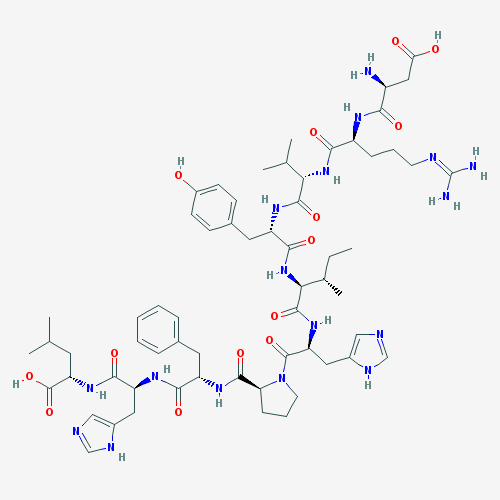
\includegraphics[width = 0.6 \textwidth]{angiotensin.png}
  \caption{Depiction of Angiotensin I. The image was taken from Pubchem \cite{pubchem}. }
\end{figure}

\subsection{Vacuum Setup}
The Angiotensin molecules are now injected from the ESI chamber to the vacuum setup via a capillary. A deflector pushes the ionized molecules towards the first set of ion funnels and a skimmer, which is followed by another funnel and a second skimmer, which focus the ion beam while collecting as many ions as possible to increase intensity. From there, the ions are guided onward with a hexapole into a quadrupole mass filter, which can be used as an ion guide too if one removes the direct voltage from the electrodes in the filter. \\
Here the ions enter the collision cell, which is another hexapole. A weak argon atmosphere allows for the ions to thermalize.
%more about cid
Also, given enough collision energy, the ions can be broken up into fragments. From the collision chamber the ions are guided via ion optics into the ICR cell, where the measurement of the spectrum will be performed. A sketch of the setup is displayed in Fig. \ref{fig_setup}.
\begin{figure}[htp!]
	\centering
	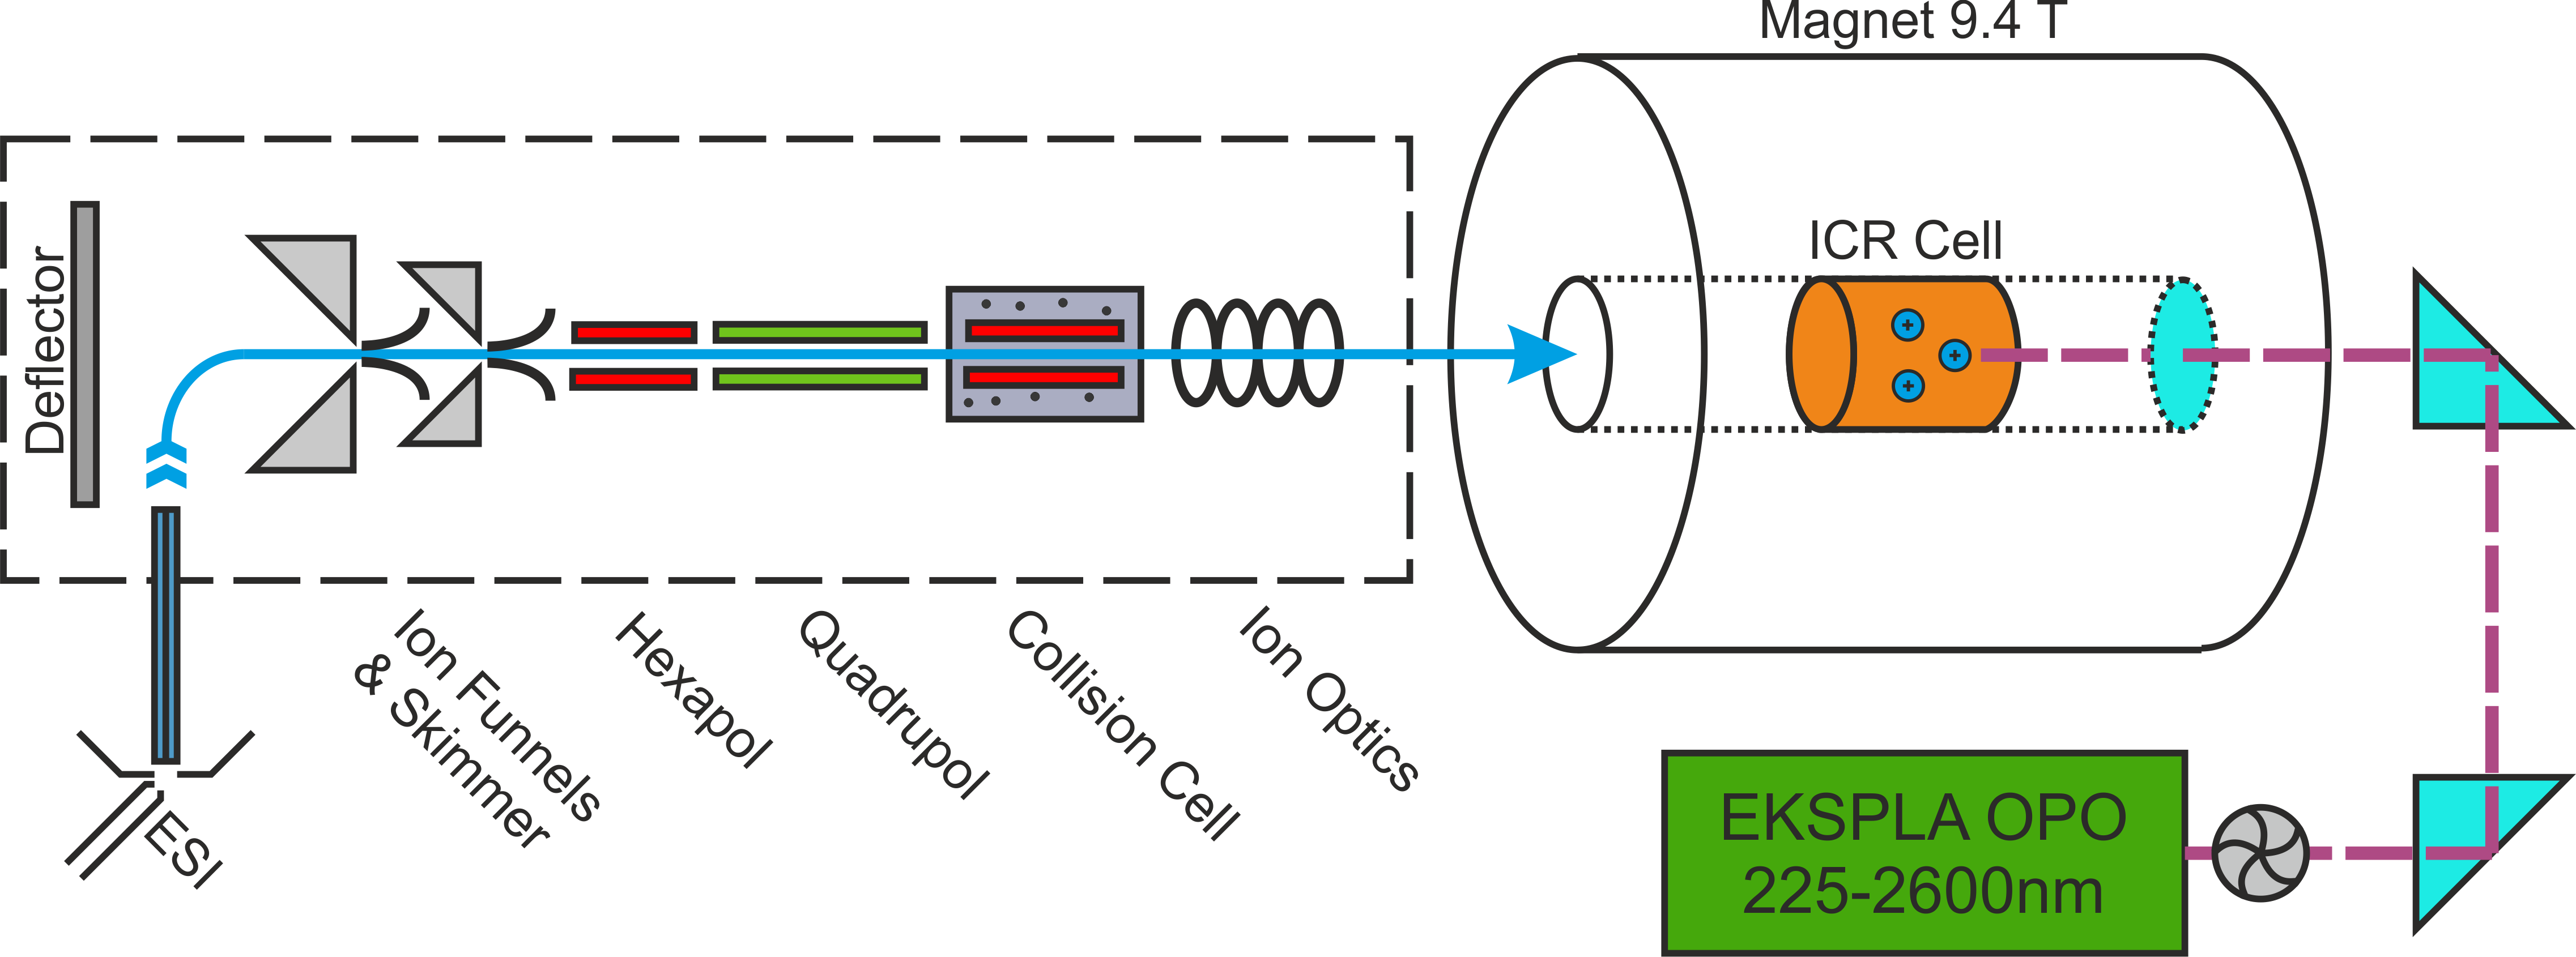
\includegraphics[width= 0.6 \textwidth]{setup.png}
	\caption{Sketch of the setup, taken from \cite{script}.}
	\label{fig_setup}
\end{figure}

\subsection{Ion Cyclotron Resonance Cell}
The ideas behind the ICR cell were already briefly laid out in Sec. \ref{sec_theory}, so here the focus is on the experimental implementation. \\
The cell used is of cylindrical shape and has two sets of electrodes to provide rotating electrical fields. Additionally, there are two more electrodes at the caps of the cylinder that generate an electric field along the direction of the magnetic field. This field has the purpose to keep the ions inside the cell, i.e. slow them down when they enter the cell, so the ion can be kept inside the ICR cell for a longer time. \\
The magnetic field in the cell is created with a superconducting \SI{9.4}{\tesla} magnet built around the ICR cell, as shown in Fig. \ref{fig_setup}.

\subsection{CID and SORI-CID}
Collision-induced dissociation is a means to study fragments of  otherwise stable ions \cite{ms_book}. The idea is that ions with low internal energy are accelerated using an electric field before colliding with neutral gas atoms (Argon in this experiment). To maintain the high-vacuum outside the collision chamber the ion beam is guided through narrow slits to enter and exit the cell. A turbomolecular pump removes gas escaping from the collision cell in order to keep the surrounding areas at high-vacuum. \\
According to \cite{ms_book}, the reaction happening upon collision can be written as
\begin{equation}
	\ch{AB+ + Ar -> AB^{+*} + Ar -> A+ + B + Ar},
\end{equation}
where in the first step kinetic energy is converted into internal energy, which causes a dissociation of the molecule in the second step. \\
Sustained off-resonance irradiation is a different method for CID, where the collision gas is introduced into the ICR cell itself. The pressure is still very low ($\sim \SI{7e-9}{\milli \bar}$), however collisions can be seen on sufficiently long timescales. As the name suggest, the frequency in the electric field is slightly off resonance, resulting in acceleration-deceleration cycles according to \cite{ms_book}. As a result the orbit does not exceed the size of the cell which would be the case for resonant excitation. This allows for multiple collisions for single ions in the cell. \\
As the acceleration is not as strong as in the resonant case the collision energies are usually smaller than \SI{10}{\electronvolt} \cite{ms_book}. Therefore dissociation routes that require little activation energy but long reaction times are usually explored with SORI-CID.

\section{Analysis}

\subsection{High resolution mass spectrum}
At the beginning of the experiment we recorder a wide range spectrum of the molecule, this can be seen in figure \ref{fullspectrum}. We can see many peak, the most prominent one is at around 430 u/e, which is the triple protonized molecule, another peak at around 650 u/e appears, this is the double protonized molecule. After the full spectrum we recorded a high-resolution mass spectrum of Angiotensin with three additional protons attached to it (\ch{C62H92N17O14^{3+}}). In order to measure the spectrum we beforehand varied parameters in the setting, i.e. voltages for example on the ESI capillary, deflector, funnels etc, to maximize the intensity of the output.
Then a spectrum was recorded over approximately \SI{40}{\minute}.\\
According to the Universal Mass Calculator \cite{umc}, this should yield an average $m/z$ ratio of \num{433.167}. This is only an average because in reality one would expect multiple peaks for different isotope combinations. As one can see in Fig. \ref{fig_hres_spectroscopy} there are in fact five peaks visible, although the last one is already hard to see. \\
Next, one can quickly estimate the resolution of the measured spectrum, so a Lorentzian curve was fitted to the highest peak in Fig. \ref{fig_hres_spectroscopy}, the fit can be seen in Fig. \ref{fig_fit_hires}. This yields a resolution of
\begin{equation}
	\frac{m}{\Delta m_\mathrm{FWHM}} = \num{1.97(3) e6}.
\end{equation}
This value is now used to calculate the error of the peaks in Fig. \ref{fig_hres_spectroscopy}. The results we extracted from said figure were \SI{432.925013 \pm 0.00021945}{\atomicmassunit \per \elementarycharge} for the first peak, \SI{433.259529 \pm 0.00021962}{\atomicmassunit \per \elementarycharge} for the second one, and \SI{433.594038 \pm 0.00021979}{\atomicmassunit \per \elementarycharge}, \SI{433.928572 \pm 0.00021996}{\atomicmassunit \per \elementarycharge}, and \SI{434.263066 \pm 0.00022013}{\atomicmassunit \per \elementarycharge} respectively for the third, forth and fifth peak, as Tab. \ref{tab_peaks_spectrum} shows.

\begin{figure}[H]
	\centering
	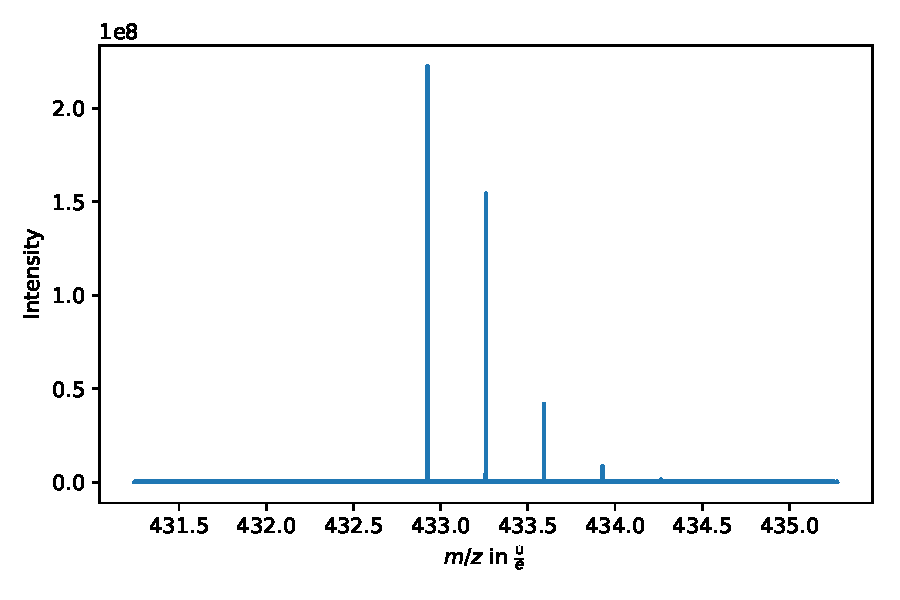
\includegraphics[width = 0.8 \textwidth]{hires_spectrum.pdf}
	\caption{Depiction of the measured data for the triple protonized Angiotensin. }
	\label{fig_hres_spectroscopy}
\end{figure}

One will notice immediately that the peaks are separated by about one third \si{\atomicmassunit \per \elementarycharge}. This is because the molecule is triple charged, meaning that the absolute difference in mass would be \SI{1}{\atomicmassunit}. In the sum formula of triple charged Angiotensin \ch{(C62H92N17O14)^{3+}} one sees that Hydrogen and Carbon appear at the highest frequency. Taking a look at Tab. \ref{tab_abundance}, one sees that the probability of having a Deuterium atom in the molecule is negligible compared to the probability of it containing a \ch{^{13}C}. The assumption the isotope spectrum is due to carbon can be backed by looking at natural abundances and the peak height in Fig. \ref{fig_hres_spectroscopy}. Using the abundances in table \ref{tab_abundance} and assuming a binomial distribution, we would expect a ratio of 1:0.67:0.22:0.048:0.008, while we measured a ratio in the peak hight of 1:0.69:0.19:0.039:0.007. One can see that the ratios are very close. The slight differences are likely due to isotopes in other elements.

\begin{figure}[htp!]
	\centering
	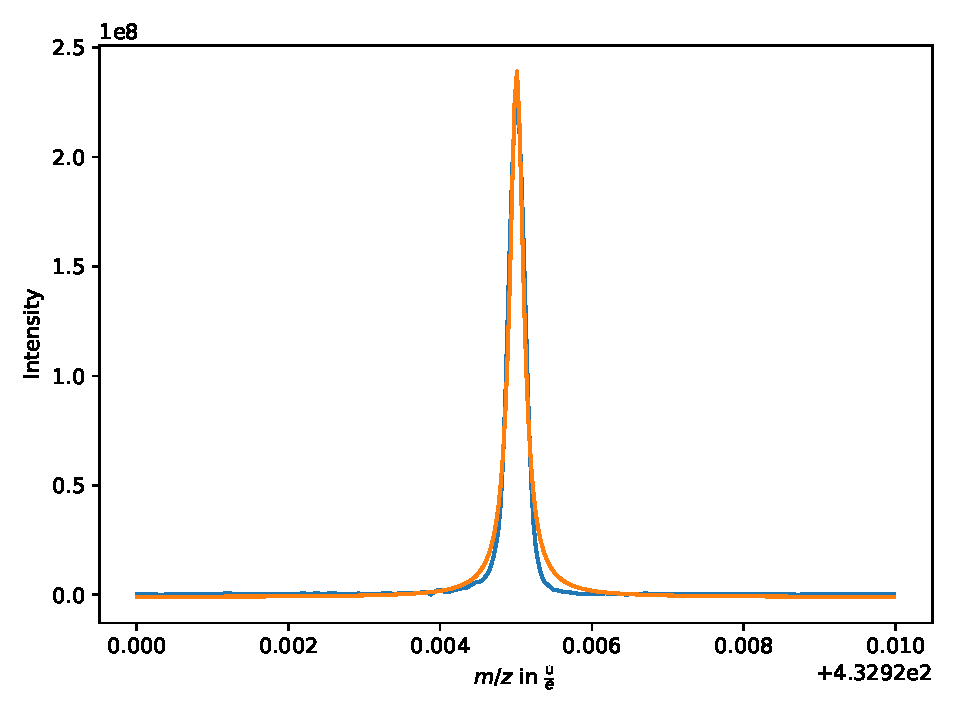
\includegraphics[width = 0.6 \textwidth]{fit_hires.pdf}
	\caption{Fitting a Lorentzian curve $y = A \frac{\gamma^2}{\gamma^2 + (x - x_0)^2} + b$ to the highest peak in the spectrum. The resulting parameters are $A = \num{2.40483457 \pm 0.0231878620 e8}$, $\gamma = \SI{1.09727221 \pm 0.0152696502 e-04}{\atomicmassunit \per \elementarycharge}$, $x_0 = \SI{432.925009(1)}{\atomicmassunit \per \elementarycharge}$, and $b = -\SI{1.07017512 \pm 0.228979314 e06}{}$. $A$ and $b$ are given in arbitrary units of intensity. }
	\label{fig_fit_hires}
\end{figure}

\begin{table}[htp!]
	\centering
	\caption{List of peak positions in Fig. \ref{fig_hres_spectroscopy}. The error is given as the FWHM of the respective peak.}
	\begin{tabular}{c | c }
		Peak number & $m/z$ (\si{\atomicmassunit \per \elementarycharge})\\ \hline
		1 & \SI{432.925013 \pm 0.00021945}{ }\\
		2 & \SI{433.259529 \pm 0.00021962}{ }\\
		3 & \SI{433.594038 \pm 0.00021979}{ }\\
		4 & \SI{433.928572 \pm 0.00021996}{ }\\
		5 & \SI{434.263066 \pm 0.00022013}{ }\\
	\end{tabular}
	\label{tab_peaks_spectrum}
\end{table}

\begin{figure}
  \centering
  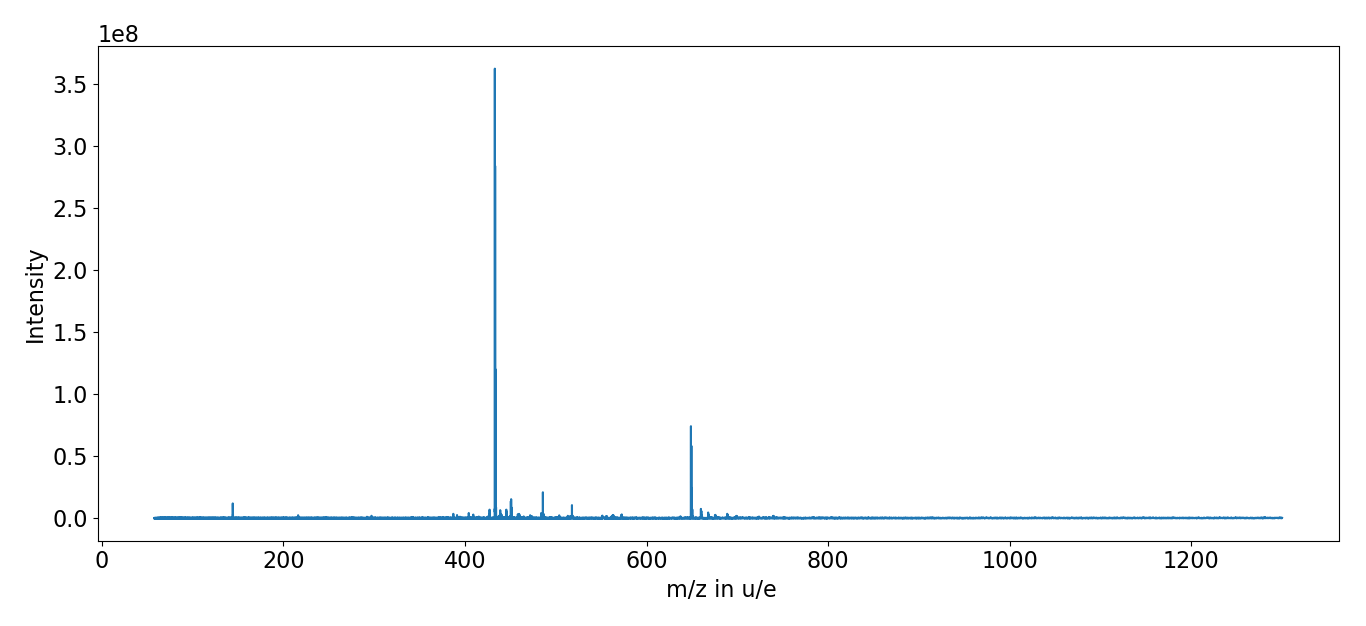
\includegraphics[width = \textwidth]{humblespectrum.png}
  \caption{Full pectrum of Angiotensin over a wide $m/z$ range. }\label{fullspectrum}
\end{figure}

\newpage

\subsection{CID fragment mass spectrum}
In this part of the experiment we produced fragments by means of CID. We analyzed the spectrum of the fragments for  different collision energy. %1018298
We changed the collision energy from 0 to 20 eV, with a step of 0.5 eV, for every measurement we took an average of twenty spectra, each one with a resolution of 44440. Then with the software Analyzze we correlated the results from every collision energy, and plotted the relative intensity of the peak as a function of the collision energy, this can be seen in figure \ref{cidcollision}.
Consequentially we have to identify the peaks which have a given relative mass, this is done by comparing all the possible $m/z$ ratios of the fragments with the measured peaks. In figure \ref{cidcollisionidentified} the identified peaks are shown with the relative fragment. Comparing figure \ref{cidcollision} and \ref{cidcollisionidentified}, we can see that we were able to identify most significant peaks apart from the orange curve (583.3002 $m/z$) with a bump around 8 eV, this is probably an internal fragmentation.
\begin{figure}[H]
	\centering
	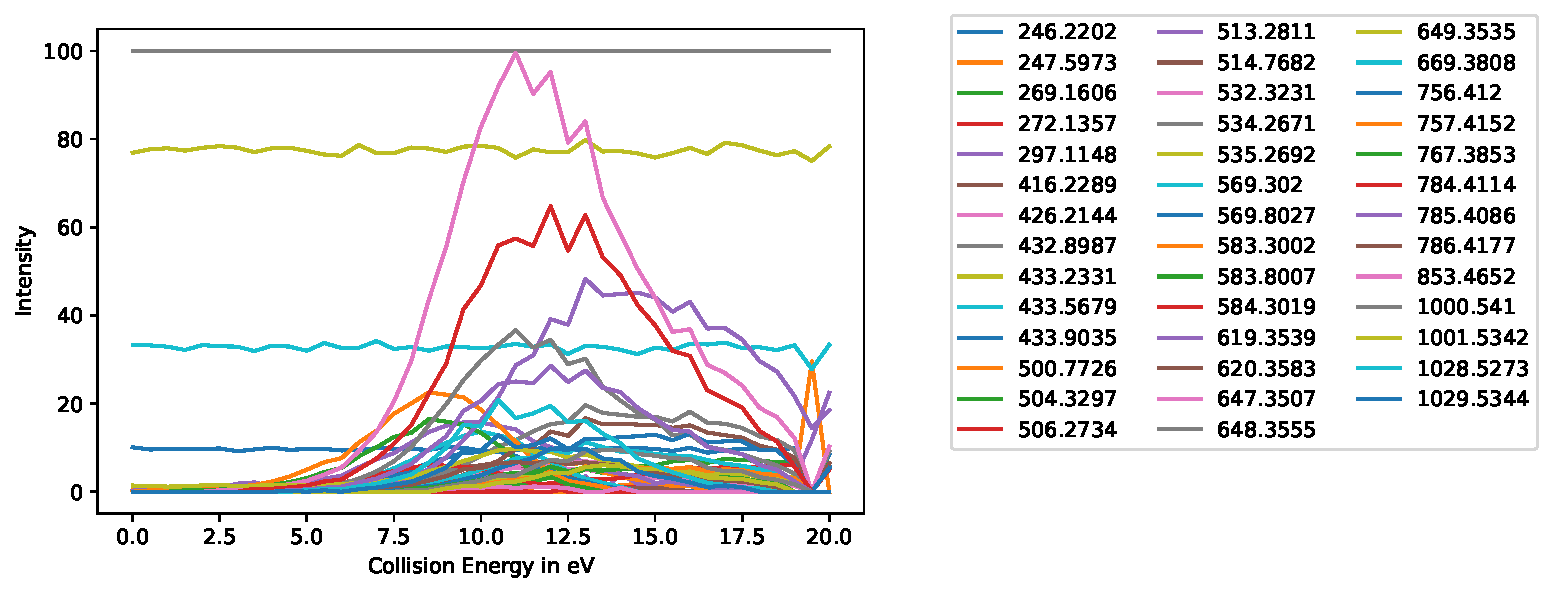
\includegraphics[width = \textwidth]{cid_collision}
	\caption{Peaks of the recorded spectrum for the CID collision. The legend indicates the ratio $m/z$}
	\label{cidcollision}
\end{figure}
\begin{figure}[H]
	\centering
	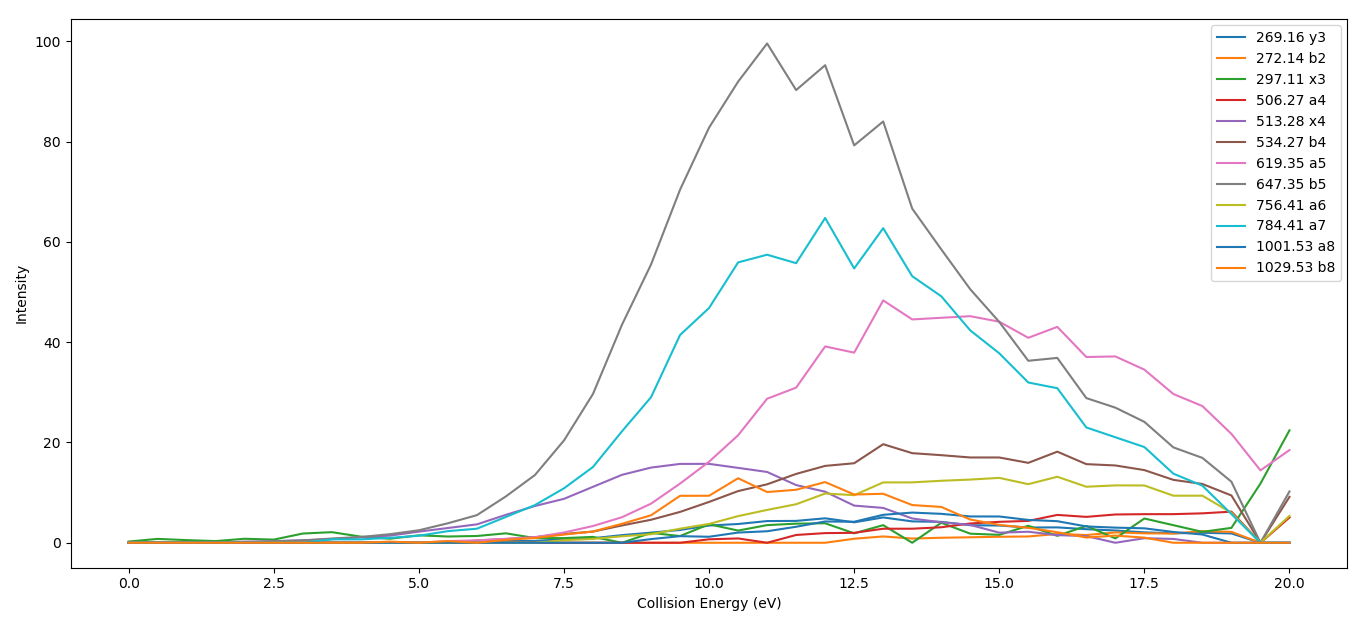
\includegraphics[width = \textwidth]{identifiedcid}
	\caption{Peaks of the identified fragments for the CID collision. The legend indicates the ratio $m/z$ and the relative fragments with the nomenclature proposed in \cite{fragmentsnomenclature}}
	\label{cidcollisionidentified}
\end{figure}
From figure \ref{cidcollisionidentified} we can notice several features of the collision. First of all, most fragments appear from 10-12 eV, with a lower collision energy, the fragments are small and not so relevant. The three most prominent peaks are from the fragments b5, a7, and a5, thus the molecule is presumably weak in these points, which we notice are approximately in the center of the molecule.  \\
Furthermore, Fig. \ref{cidcollision} shows 4 more or less constant lines. We assume these are still intact Angiotensin molecules. Presumably the difference in intensity between those lines is due to the natural abundance in isotopes, as was the case in the discussion of the high-resolution spectrum. \\
In Tab. \ref{tab_cid_candidates} we listed all $m/z$ ratios that are either above $20$ in intensity in Fig. \ref{cidcollisionidentified} or could be assigned to a fragment by a self-built program. As one can see, we were able to identify a fragmentation candidate for most of the peaks, however some remain unassigned. We are not sure whether they are multiply charged fragments, but it would seem unlikely as their actual mass would then be above \SI{1000}{\atomicmassunit} for all the unidentified fragments in Tab. \ref{tab_cid_candidates}. Further if could be the case that a either two fragments reconnected to for a unknown new fragment, but that would probably be unlikely.

\begin{table}
	\centering
	\caption{List of detected $m/z$-ratios and fragmentation candidates.  }
	\begin{tabular}{c | c | c}
		$m / z$ & candidate & formula \\ \hline
		$247.60$ & c2 + y6 & \ch{C14H18NO3+} \\
		$269.16$ & y3 & \ch{(C12H21N4O3)+} \\
		$272.14$ & b2 & \ch{(C10H18N5O4)+} \\
		$297.11$ & x3 & \ch{(C13H21N4O4)+} \\
		$506.27$ & int4 & \\
		$513.28$ & y4 & \ch{(C26H37N6O5)+} \\
		$534.27$ & b4 & \ch{(C24H36N7O7)+} \\
		$583.30$ & & \\
		$619.35$ & int5 & \\
		$647.35$ & b5 & \ch{(C30H47N8O8)+}\\
		$648.36$ & b5 with isotope & \\
		$756.41$ & a6 & \ch{(C35H54N11O8)+} \\
		$784.41$ & b6 & \ch{(C36H54N11O9)+}\\
		$785.41$ & b6 with isotope & \\
		$1001.53$ & a8 & \ch{(C49H70N13O10)+}\\
		$1028.52$ & b8 & \ch{(C50H70N13O11)+} \\
		$1029.53$ & b8 with isotope & \\
	\end{tabular}
	\label{tab_cid_candidates}
\end{table}

\subsection{SORI-CID fragment mass spectrum}
For the last part of the experiment, we induced the fragmentation with a different technique, the SORI. The measurements were done with the same procedure and same settings. The analysis was done again with the Analyzze software. In figure \ref{soricollision} the results are shown, here the peaks are represented as a function of the SORI power.


\begin{figure}[H]
	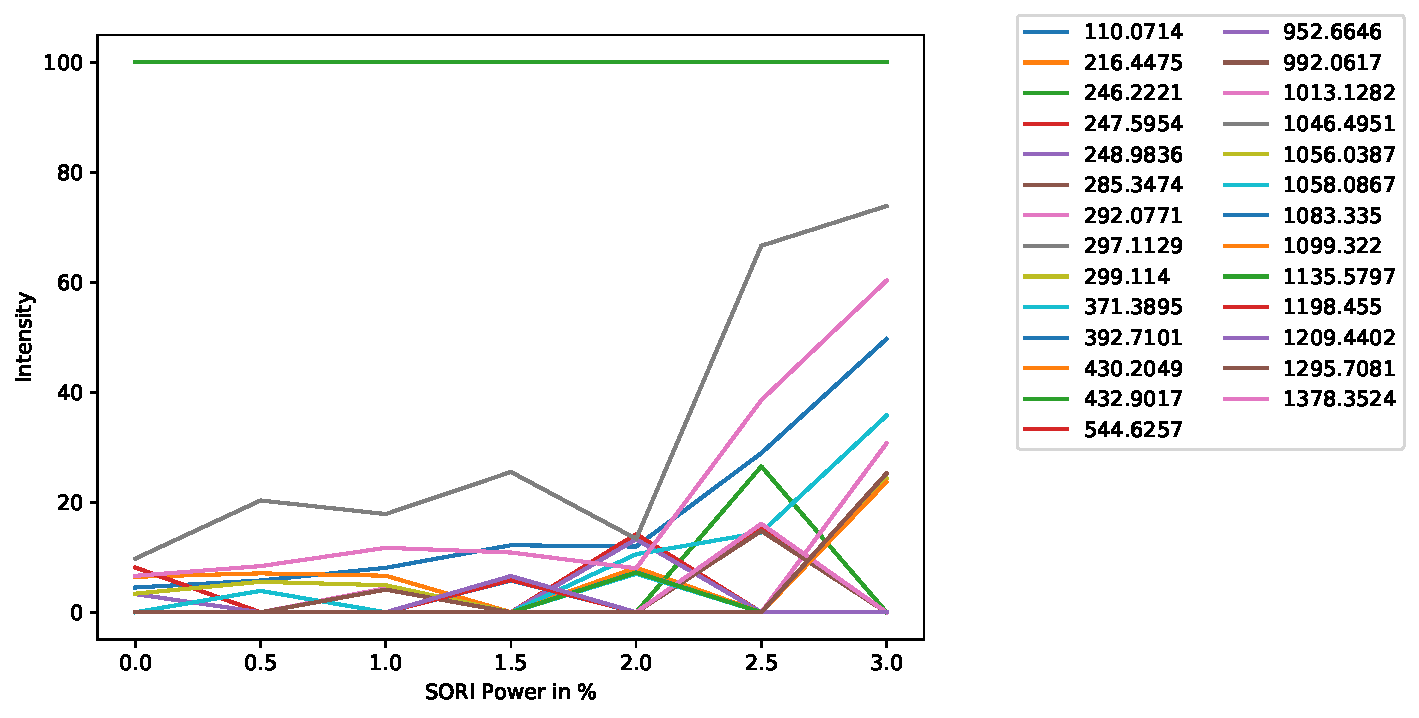
\includegraphics[width = \textwidth]{sori_cid.pdf}
	\caption{Peaks from the SORI collision experiment. The legend indicates the ratio $m/z$.}
	\label{soricollision}
\end{figure}
There are not a lot of meaningful peaks, probably because the SORI power is too low in our measurements. Anyway at 3.0\% SORI power we start to see increasing intensity at several $m/z$-ratios, and we tried to identify the corresponding fragments. In figure \ref{soriidentified} the peaks we could identify with our program are shown. Other significant $m/z$-ratios were looked at in Tab. \ref{tab_sori}. However, we were not able to identify all fragments, as is shown in the table. The problem might be that since there are multiple collisions in SORI-CID, there should be multiple fragmentations. If the fragmentation does not happen on the main string of the molecule, but on a side group of a amino acid, then there are many different possibilities for fragmentation, which we could not cover by hand. One might be able to brute-force the respective combinations for the $m/z$ ratios by trying all possible combinations of atoms from the original molecule, Angiotensin (\ch{C62H89N17O14}), but that would exceed our programming capabilities.

\begin{figure}[H]
	\centering
	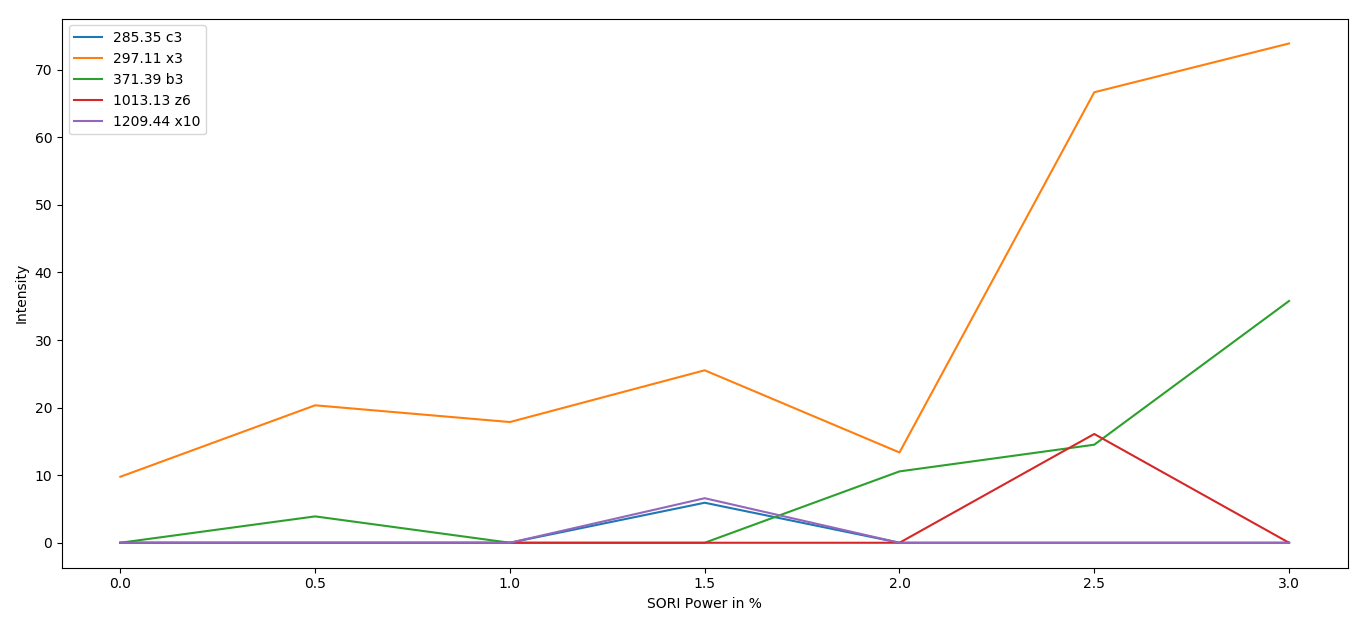
\includegraphics[width = \textwidth]{identifiedsori.png}
	\caption{Peaks of the identified SORI fragments. The legend indicates the ratio $m/z$ and the relative fragments with the nomenclature proposed in \cite{fragmentsnomenclature}.}
	\label{soriidentified}
\end{figure}

\begin{table}
	\centering
	\caption{List of detected $m/z$-ratios and fragmentation candidates.}
	\label{tab_sori}
	\begin{tabular}{c | c | c}
		$m/z$ & candidate & formula \\ \hline
		$110.07$ & b5+x4 & \ch{(C5H7N3)+}\\
		$292.08$ & & \\
		$297.11$ & & \\
		$371.39$ & b3 & \ch{(C15H27N6O5)+} \\
		$432.90$ & Angiotensin & \ch{(C62H92N17O14)^{3+}}\\
		$1056.03$ & & \\
		$1099.32$ & & \\
	\end{tabular}
	
\end{table}

\section{Conclusion}
In this experiment we performed Fourier Transform Ion Cyclotron Resonance Mass Spectrometry on the molecule Angiotensin I. First we took an high resolution spectrum of the molecule to measure the resolution of the mass spectrometer. We were able to distinguish isotopes, which are probably due to Carbon-13. Then in the last part of the experiment we performed collision experiments with two different techniques, CID and SORI collision. In both cases we studied the fragments for the collision and we identified most of the fragments, but with SORI internal fragmentations are more likely to occur, and they are more difficult to identify. With more time it would be possible to bruteforce every possible combination and perhaps identify the remaining fragments.



\begin{thebibliography}{99}
\bibitem{electrospray}
\textsc{Simon J. Gaskell}, JOURNAL OF MASS SPECTROMETRY, VOL. 32, 677È688 (1997), \textit{Electrospray : Principles and Practice}, Michael Barber Centre for Mass Spectrometry, Department of Chemistry, UMIST, Manchester M60 1QD, UK

\bibitem{primer}
\textsc{Alan G. Marshall, Christopher L. Hendrickson, George S. Jackson}, \textit{FOURIER TRANSFORM ION CYCLOTRON RESONANCE MASS SPECTROMETRY: A PRIMER}, Center for Interdisciplinary Magnetic Resonance, National High Magnetic Field Laboratory, Florida State University, 1800 East Paul Dirac Dr., Tallahassee

\bibitem{ms_book}
\textsc{Jürgen H. Gross}, \textit{Mass Spectrometry}, Springer, 2nd Edition, 2011

\bibitem{fragmentsnomenclature}
\textsc{Roepstroff P, Fohlman J}, \textit{Proposal for a common nomenclature for sequence ions in mass spectra of peptides}, Biomed. Maa Spectrom. 11 (11): 601 (1984)

\bibitem{pubchem}
\textit{Pubchem Open Chemistry Database}, \url{https://pubchem.ncbi.nlm.nih.gov/compound/angiotensin_i#section=Top}

\bibitem{script}
\textsc{Christian van der Linde}, \textit{Skriptum High Resolution Mass Spectrometry}, Universität Innsbruck

\bibitem{abundance}
\textit{Table of Isotopic Masses and Natural Abundances}, North Carolina State University, \url{https://chemistry.sciences.ncsu.edu/msf/pdf/IsotopicMass_NaturalAbundance.pdf}

\bibitem{umc}
\textsc{Matthias Letzel}, \textit{Universal Mass Calculator - Student Edition}, Universität Münster, \url{https://www.uni-muenster.de/Chemie.oc/ms/downloads.html}

\end{thebibliography}

\begin{appendices}
\begin{table}[htp!]
	\centering
	\caption{List of possible breaking points in peptide fragmentation notation of Roepstorff and Fohlman. The data was obtained with UMC \cite{umc}. }
	\begin{tabular}{c | c | c | c | c | c}
		Fragment & mass (${\mathrm{u}}/{z}$) & Fragment & mass (${\mathrm{u}}/{z}$) & Fragment & mass (${\mathrm{u}}/{z}$) \\ \hline
		$a_1$ & $88.085$ & $b_1$ & $116.095$ & $c_1$ & $131.11$ \\
		$a_2$ & $244.271$ & $b_2$ & $272.281$ & $c_2$ & $287.296$ \\
		$a_3$ & $343.402$ & $b_3$ & $371.412$ & $c_3$ & $286.427$ \\
		$a_4$ & $506.567$ & $b_4$ & $534.586$ & $c_4$ & $549.6$ \\
		$a_5$ & $619.733$ & $b_5$ & $647.744$ & $c_5$ & $662.758$ \\
		$a_6$ & $756.873$ & $b_6$ & $784.883$ & $c_6$ &  \\
		$a_7$ & $784.883$ & $b_7$ & $881.998$ & $c_7$ & $897.013$ \\
		$a_8$ & $1001.163$ & $b_8$ & $1029.173$ & $c_8$ & $1044.187$ \\
		$a_9$ & $1138.301$ & $b_9$ & $1166.312$ & $c_9$ & $1181.327$ \\
		$a_{10}$ & $1251.46$ & $b_{10}$ & $1279.47$ & $c_{10}$ &  \\
		$x_{1}$ & $47.03$ & $y_{1}$ & $19.023$ & $z_{1}$ & $117.166$ \\
    $x_{2}$ & $160.192$ & $y_{2}$ & $132.181$ & $z_{2}$ & $254.306$ \\
    $x_{3}$ & $297.32$ & $y_{3}$ & $269.31$ & $z_{3}$ & $401.479$ \\
    $x_{4}$ & $513.60$ & $y_{4}$ & $416.49$ & $z_{4}$ &  \\
    $x_{5}$ & $541.61$ & $y_{5}$ & $513.60$ & $z_{5}$ & $635.734$ \\
    $x_{6}$ & $678.76$ & $y_{6}$ & $650.74$ & $z_{6}$ & $748.892$ \\
    $x_{7}$ & $791.92$ & $y_{7}$ & $763.90$ & $z_{7}$ & $912.065$ \\
    $x_{8}$ & $955.09$ & $y_{8}$ & $927.08$ & $z_{8}$ & $1011.196$ \\
    $x_{9}$ & $1054.222$ & $y_{9}$ & $1026.212$ & $z_{9}$ & $1167.382$ \\
    $x_{10}$ & $1210.408$ & $y_{10}$ & $1182.398$ & $z_{10}$ & $$ \\
	\end{tabular}
	\label{tab_fragments}
\end{table}

\begin{table}[htp!]
	\centering
	\caption{List of natural abundance of isotopes of Hydrogen, Carbon, Nitrogen, and Oxygen. The data was taken from \cite{abundance}. }
	\begin{tabular}{c | c }
		Isotope & natural abundance in \% \\ \hline
		\ch{^1H} & 99.9885 \\
		\ch{^2H} & 0.0115 \\ \hline
		\ch{^{12}C} & 98.93  \\
		\ch{^{13}C} & 1.07  \\ \hline
		\ch{^{14}N} & 99.632 \\
		\ch{^{15}N} & 0.368 \\ \hline
		\ch{^{16}O} & 99.757 \\
		\ch{^{17}O} & 0.038 \\
		\ch{^{18}O} & 0.205 \\
	\end{tabular}
	\label{tab_abundance}
\end{table}
\end{appendices}

\end{document}
